Der Server, der im lokalen Netz auf einem Raspberry Pi läuft, soll für die manuellen Tests der Ladesäule benutzt werden.
Dieser Server wird benutzt um die komplexeren Testfälle nachzubilden oder neue Funktionalitäten, die mit Hardware interagieren, zu testen.
Der Server kann bei der Präsentation der Funktionalitäten genutzt werden.

Die Anforderungen an den Server sind:
\begin{itemize}
    \item Der Server soll eine OCPP1.6 Schnittstelle besitzen.
    \item Der Nutzer soll in der Lage sein den Server zu parametrieren (z.B. einen neuen Benutzer hinterlegen)
    \item Der Nutzer soll in der Lage sein die Nachrichten an die Ladesäule manuell verschicken zu können
\end{itemize}

Die nachfolgende Abbildung \ref{fig:summaryDiagrammStandaloneWithDB} ist ein Übersichtdiagramm der Standalone-Anwendung mit Datenbank.
\begin{figure}[H]
    \centering
    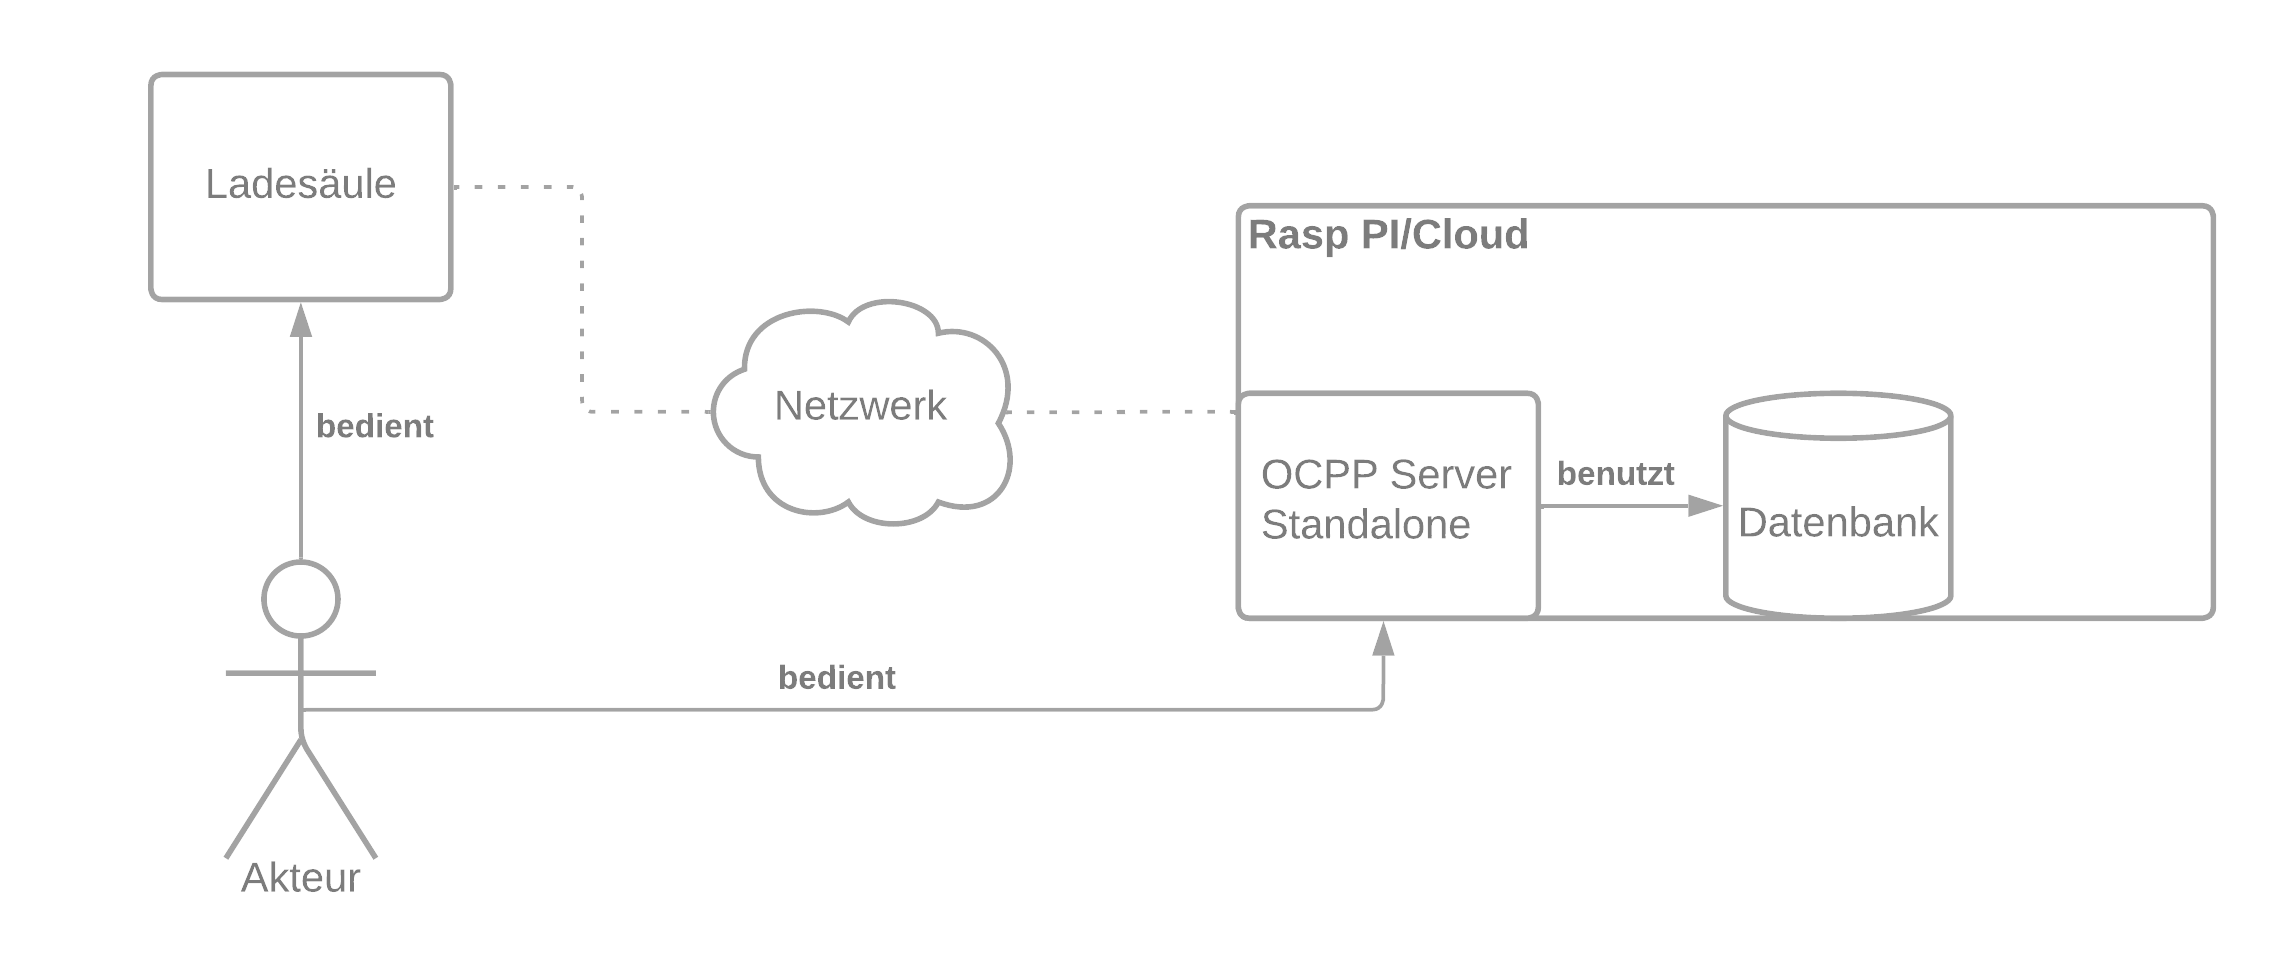
\includegraphics[width=1\textwidth]{./images/OCPP Server Standalone mit DB.png}
    \caption[Übersichtdiagramm der Standalone-Anwendung mit Datenbank]{Übersichtdiagramm der Standalone-Anwendung mit Datenbank}
    \label{fig:summaryDiagrammStandaloneWithDB}
\end{figure}